%%%%%%%%%%%%%%%%%%%%%%%%%%%%%%%%%%%%%%%%%%%%%%%%%%%%%%%%%%%%%%%%%%%%%%%%%%%%%
%%%
%%% File: thesis.tex, version 0.1, May 2010
%%%
%%% =============================================
%%% This file contains a template that can be used with the package
%%% cs.sty and LaTeX2e to produce a thesis that meets the requirements
%%% of the Computer Science Department from the Technical University of Cluj-Napoca
%%%%%%%%%%%%%%%%%%%%%%%%%%%%%%%%%%%%%%%%%%%%%%%%%%%%%%%%%%%%%%%%%%%%%%%%%%%%%

\documentclass[12pt,a4paper,twoside]{report}
\usepackage{cs}
\usepackage{times}
\usepackage{graphicx}
\usepackage{subfigure}
\usepackage{latexsym}
\usepackage{amsmath,amsbsy}
\usepackage{amssymb}
\usepackage[matrix,arrow]{xy}
\usepackage{ae,aecompl}
\usepackage{amstext}
\usepackage{graphics}
\usepackage{ae,aecompl}
\usepackage{algorithm}
\usepackage{algorithmic}
\usepackage{color}
\usepackage{listings}

\usepackage{tabularx}

\usepackage{hyperref}

\usepackage[english,romanian]{babel}
\usepackage{pgfpages}

\usepackage{ucs}
\usepackage[utf8x]{inputenc}
\usepackage[T1]{fontenc}



\lstset{%
    language=C,
    basicstyle=\ttfamily,
    keywordstyle=\bfseries,
    commentstyle=\itshape,
    escapechar=\#,
    emphstyle=\bfseries\color{red}
 }


\usepackage{ifpdf}

\graphicspath{{figures/}}
\ifpdf
  \DeclareGraphicsExtensions{.pdf,.jpeg,.jpg,.png}
\else
  \DeclareGraphicsExtensions{.eps}
\fi

% \mastersthesis
\diplomathesis
% \leftchapter
\centerchapter
% \rightchapter
\singlespace
% \oneandhalfspace
% \doublespace

\renewcommand{\thesisauthor}{Mureșan Cătălin-Gabriel}% Your name.
\renewcommand{\thesismonth}{Iulie}     %% Your month of graduation.
\renewcommand{\thesisyear}{2014}      %% Your year of graduation.
\renewcommand{\thesistitle}{Mediu de învățare 3D}
\renewcommand{\thesissupervisor}{Conf.dr.ing. Mihai DAMIAN  , Prof.Dr.Ing. Liviu MICLEA}

%\renewcommand{\thesisdedication}{P'arin'tilor mei}

\begin{document}

\begin{titlepage}
\begin{center}
UNIVERSITATEA TEHNICĂ DIN CLUJ-NAPOCA\\
FACULTATEA DE AUTOMATICĂ ȘI CALCULATOARE\\
DEPARTAMENTUL AUTOMATICĂ\\

\vspace{6cm}

\Huge {\textbf{Mediu de învățare 3D}\\}
\vspace {1cm}
\Large \textbf{Lucrare de disertație}\\

\vspace{2cm}

\large Absolvent \\ \textbf{Mureșan Cătălin-Gabriel}\\

\vspace{\stretch{1}}
Iulie, 2014\\
\end{center}
\end{titlepage}

\begin{titlepage}
\phantom{1}
\end{titlepage}


\begin{titlepage}

\begin{center}
UNIVERSITATEA TEHNICĂ DIN CLUJ-NAPOCA\\
FACULTATEA DE AUTOMATICĂ ȘI CALCULATOARE\\
DEPARTAMENTUL CALCULATOARE\\

\vspace{1cm}

\newcolumntype{R}{>{\raggedleft\arraybackslash}X}%
\begin{tabularx}{\textwidth}{lR}
DECAN & DIRECTOR DEPARTAMENT \\
Prof.Dr.Ing. Liviu MICLEA & Prof.Dr.Ing. Rodica POTOLEA\\
\end{tabularx}

\vspace {3cm}

\Huge \textbf{Mediu de învățare 3D}\\
\vspace {1cm}
\Large \textbf{Lucrare de disertație}\\
\vspace{1cm}

\end{center}

% \vspace{1cm}

\begin{flushleft}
\begin{enumerate}
 \item Absolvent: Mureșan Cătălin-Gabriel

 \item Coordonator științific (1): Conf.dr.ing. Mihai DAMIAN\\
 \item Coordonator științific (2): Prof.Dr.Ing. Liviu MICLEA
 \item Conținutul lucrării: Pagina de prezentare, aprecierile coordonatorului, titlul capitolului 1, titlul capitolului 2, \dots, titlul capitolului n, bibliografie, anexe, CD.

 \item Locul documentării: UTCN, Cluj-Napoca

 \item Consultanți: \dotfill

 \item Data emiterii temei: \dotfill

 \item Data predării: \dotfill
\end{enumerate}

\end{flushleft}

\vspace{0.5cm}

\begin{center}

\newcolumntype{R}{>{\raggedleft\arraybackslash}X}%
\begin{tabularx}{\textwidth}{lR}
Semnătură coordonator & Semnătură absolvent \\
Conf.dr.ing. Mihai DAMIAN\\Prof.Dr.Ing. Liviu MICLEA & Mureșan Cătălin-Gabriel \\
\end{tabularx}

\vspace{\stretch{1}}
Iulie, 2014\\

\end{center}

\end{titlepage}


\begin{titlepage}
\phantom{1}
\end{titlepage}


\begin{titlepage}

\begin{center}
UNIVERSITATEA TEHNICĂ DIN CLUJ-NAPOCA\\
FACULTATEA DE AUTOMATICĂ ȘI CALCULATOARE\\
DEPARTAMENTUL CALCULATOARE\\
\end{center}

\vspace{4cm}

\begin{center}
\textbf{Declarție pe proprie răspundere privind \\ autenticitatea lucrării de disertație}

\end{center}

\vspace{1cm}

Subsemnatul \textit{Mureșan Cătălin-Gabriel}, legitimat cu \textit{CI} seria \textit{KT} numărul \textit{771623}, CNP \textit{1820513013911}, autorul lucrării \textit{Mediu de învățare 3D} elaborată în vederea susținerii examenului de finalizare a studiilor de masterat la Facultatea de Automatică și Calculatoare, Departamentul Automatica, Specializarea \textit{Informatică Aplicată} din cadrul Universității Tehnice din Cluj-Napoca, sesiunea \textit{Iulie} a anului univeristar \textit{2013/2014}, declar pe proprie răspundere, că această lucrare este rezultatul propriei mele activități intelectuale, pe baza cercetărilor mele și pe baza informatiilor obținute din surse care au fost citate în textul lucrării și în bibliografie.

Declar că această lucrare nu conține porțiuni plagiate, iar sursele bibliografice au fost folosite cu respectarea legislației române și a convențiilor internaționale privind drepturile de autor.

Declar, de asemenea, că această lucrare  nu a mai fost prezentată în fața unei alte comisii de examen de licență sau disertație.

În cazul constatării ulterioare a unor declarații false, voi suporta sancțiunile administrative, respectiv, \textit{anularea examenului de disertație}.


\vspace{3cm}

\newcolumntype{R}{>{\raggedleft\arraybackslash}X}%
\begin{tabularx}{\textwidth}{lR}
Cluj-Napoca & PRENUME NUME\\
data  &    Semnătură absolvent \\
\end{tabularx}


\end{titlepage}


\begin{titlepage}
\phantom{1}
\end{titlepage}


%\pagestyle{headings}

\newenvironment{definition}[1][Definiție.]{\begin{trivlist}
\item[\hskip \labelsep {\bfseries #1}]}{\end{trivlist}}

% ABSTRACT
\begin{abstract}
\par Progresul rapid în domeniul I.T.\& C și scăderea prețurilor componentelor hardware performante a făcut fezabilă aplicarea metodei de învațare in medii virtuale 3D în oricare treaptă a sistemului educațional.
Într-un mediu virtual tridimensional, obiectele studiate sunt reprezentate prin coordonate ce descriu forma și pozitionarea lor în spațiu, apropiind astfel modul de reprezentare de cel al obiectelor din lumea reală. Utilizatorii se pot poziționa în orice punct al spațiului virtual, fapt care le va permite să studieze obiectele din orice unghi, lucru dificil de realizat cu programele informatice cu redare 2D. De asemenea o parte dintre obiectele virtuale pot fi programate să răspundă la acțiunea utilizatorului, conducând la sporirea gradului de implicare a utilizatorului, cu rezultate benefice în procesul de învățare. \\
\par Foarte importantă este siguranța și costul redus. Utilizatorii au șansa de a efectua activități care ar fi altfel foarte costisitore pentru instituțiile implicate în procesul de educare, sau în medii cu grad mare de risc. În mediile de învățare 3D se pot repeta în siguranță proceduri care nu sunt tolerante la erori, precum operațiile chirurgicale sau controlul proceselor într-o centrala nucleara. \\
\par În această lucrare sunt sunt identificate elementele necesare pentru implementarea unui program informatic reprezentând un asemenea mediu de învațare 3D, care să ruleze în sistemul de operare Linux, și se va face descriere a arhitecturii aplicației. Această lucrare va conține și codul sursă cu comentarii pentru a putea fi folosită ca exemplu pentru programtorii și designerii de medii virtuale aplicate în educație.
\end{abstract}

\begin{titlepage}
\phantom{1}
\end{titlepage}



%\thesistitle                    %% Generate the title page.
%\authordeclarationpage                %% Generate the declaration page.

\pagenumbering{roman}
\setcounter{page}{1}

\tableofcontents
\newpage

\listoftables
\listoffigures

\clearpage
\newpage

\pagenumbering{arabic}
\setcounter{page}{1}


%\setcounter{page}{\value{page}}
\chapter{Introducere}
\label{cap:Introducere}
%\setcounter{page}{7}
%\addtocounter{page}{6}
\pagestyle{headings}
\section{Introducere}
\par \textbf{Acest capitol definește în secțiunea 1.2 problema adresată, fiind subliniați principalii piloni ai problemei: costul serviciilor educaționale și în special complexitatea și costul ridicat al soluțiilor existente ce implică tehnologia mediilor de învățare 3D. Secțiunea 1.3 este un enunț al soluției ce se dorește a fi oferită în această lucrare. Secțiunea 1.4 subliniază etaplele studiului iar secțiunea 1.5 tratează în linii mari teorii referitoare la mediile de învățare 3D și la învățare în general, teorii ce vor avea influență asupra produsului final (applicația informatică).}
\section{Problema adresată}
\par Asigurarea unui învățămînt de calitate poate implica costuri semnificative pentru diversele instituții sau organizații care oferă asemenea servicii, în special când mediul optim de învățare presupune colaborarea, întreprinderea de experimente multiple sau lucrul în medii cu risc ridicat. De asemenea, în unele cazuri, instruirea poate avea loc în medii simulate al căror cost de construire și folosire ar fi mult prea mare.
\section{Motivație}
\par Ca răspuns la complexitatea și costul soluțiilor existente, se dorește realizarea unei aplicații reprezentând o un mediu virtual 3D; o aplicație de dimensiuni reduse dar care poate fi cu ușurință extinsă și completată cu noi elemente reprezentând: experimente de laborator virtual, diverse forme de reprezentare în forma grafica 3D a cunoștințelor, spații virtuale pentru desfașurarea de activități educative (muzee, săli de conferință virtuală) etc. 
O asemenea aplicație va avea se va dezvolta în două module: client și server, ambele dinamice, ușor de extins și care să se constituie o mini platformă pe care alți programatori să poată construi cu minim efort lumi virtuale orientate spre livrarea conținutului educativ intr-o formă cât mai atragatoare pentru utilizatori.
\par Aplicația informatică va rula sub GNU/Linux, pentru inplementarea acesteia se vor folosi doar unelte și bibilioteci software dezvoltate de comunitățile free software / open source. Codul sursa va fi eliberat cu o licență liberă.
\section{Descrierea studiului pe capitole}
\par În \textbf{\textit{Capitolul 1}} (capitolul curent) se pune accentul pe descrierea nevoii instituțiilor furnizoare de servicii educațional de unelte moderne pentru îndeplinirea obiectivelor lor specifice și pe lipsa de alternative care să indeplinească  \textbf{simultan} următoarele aspecte: libertatea codului (open source / free software), dimensiune redusă și modularitate ridicată, costuri minime. Se afirmă obiectivul creării unui program liber (free/open source) ușor de menținut și extins reprezentând o lume virtuală 3D. Definițiile și conceptele teoriei învățării in medii virtuale încheie capitolul 1.
\par În \textbf{\textit{Capitolul 2}} sunt enumerate obiectivele cercetării.
\par În \textbf{\textit{Capitolul 3}} sunt prezentate specificațiile generale ale lucrării de cercetare, atât obiectivele minimale care vor trebui atinse până la definitivarea studiului cât și obiectivele potențiale de atins în cazul extinderii lucrării.
\par În \textbf{\textit{Capitolul 4}} se analizează sistemul în întregime prin descrierea ansamblului \textit{client-server}. Se decide design-ul  sistemului și se argumentează alegerea făcută prin testele anterior stabilite.
\par În \textbf{\textit{Capitolul 5}} se realizează un studiu amănunțit al aplicației \textit{server} din sistem. Se decide design-ul aplicației, se efectuează teste și se decid aspectele tehnice referitoare la implementarea aplicației: limbajul folosit pentru implementare, librării software folosite, algoritmi și metode de implementare.
\par În \textbf{\textit{Capitolul 6}} se realizează un studiu amănunțit al aplicației \textit{client} din sistem. Se decide design-ul aplicației, se efectuează teste și se decid aspectele tehnice referitoare la implementarea aplicației: limbajul folosit pentru implementare, librării software folosite, algoritmi și metode de implementare.
\par În \textbf{\textit{Capitolul 7}} sunt prezentate concluziile.
\section{Învațarea și mediile 3D. Concepte relevante.}
\par În mare masură, soluția tuturor acestor probleme se găsește în mediile de învățare virtuale cu redare 3D, datorită unor caracterisici care le califică ca și cadru (în unele cazuri ideal) de învățare. Unele dintre cele mai importante caracteristici ale mediilor de învățare cu redare tridimensionala sunt: capacitatea de a simula orice spațiu fizic, de a intermedia interacțiunea dintre diverse persoane aflate în zone geografice diferite și oferta de unelte de observare și măsurare a performanțelor sau a progresului participanților la procesul de învățare și faptul ca orice resursă virtuală poate fi refolosită fară costuri suplimentare.
\par O analiză a autorilor Wann și Mon Williams oferă o descriere a mediilor tridimensionale ca medii ce ”valorifică aspectele naturale ale percepției umane prin extinderea informațiilor vizuale în trei dimensiuni spațiale și care poate suplimenta aceasta informație cu alți stimuli și modificari temporale”\cite{C01} și care ”permit interacțiunea utilizatorului cu obiectele redate”\cite{C01}. Se pot astfel deduce trei elemente care disting mediile de învățare 3D de alte medii de învățare virtuale. 	Mai detaliat, mediile virtuale tridimensionale sunt medii grafice ce crează impresia de spațiu 3D, în care utilizatorul controlează caractere generate de computer (avatare), caractere care îi reprezintă în timp ce interacționează cu mediul sau cu alți utilizatori. Acestea pot contribui la sistemul educațional prin facilitarea colaborării, comunicării și experimentării. Prin oferirea unui surogat al realității, mediile de învățare pot crea percepția de existență a utilizatorului în mediul simulat. 
\par În psihologie și educație, învățarea este definită ca fiind procesul care aduce împreună experiența cognitivă, emoțională și influența de mediu, pentru acumularea, îmbunatațirea sau schimbarea cunoștințelor, abilităților sau a concepției despre lume a unui individ.[C02]
\par Clasificarea metodelor de învățare, stabilită de Frederic Vester[c03] : învățarea auditivă, învățarea vizuală, învățarea tactilă, învățarea cognitivă ( prin intelect ). Prin această metodă de clasificare F. Vester, neagă efortul intelectual pentru primele trei tipuri, acest efort fiind atribuit învățării cognitive. Deși nu poate fi în totalitate adevărat, fiecare dintre noi am putut experimenta reducerea 'consumului' intelectual atunci când am învățat folosindu-ne de materiale didactice cu vizuale sau auditive. Personele de toate vârstele învață cel mai bine atunci cînd sunt implicate în experiențe semnificative. Învățarea are loc atunci când mintea este capabilă să pună la un loc informațiile primite de la toate simțurile și să le coreleze cu experințele trecute. Prin folosirea mai multor simțuri pentru a învăța se poate da mai mult sens procesului de acumulare. Copii în mod natural învață folosindu-se de toate simțurile în cel mai eficient mod posibil.
\par Valoarea unui mediu 3D bine construit constă în faptul ca poate antrena simțul vizual al utilizatorului, cu îmbunătățirea rezultatelor. 
\chapter{Obiectivele cercetării}
\section{Introducere}
\par \textbf{În secțiunea 2.2 se definește obiectivul lucrării și se enumeră etapele necesare îndeplinirii obiectivului. Motivația alegerii acestui obiectiv este prezentată, în secțiunea 2.3, cu argumente de ordin estetic referitoare la calitatea prezentării materialelor educative în redare tridimensională cât și cu argumente practice referitoare la utilitatea aplicației software rezultate. Dorința autorului de a dezvolta o aplicație din categoria free software / open source este evidentă și este în sine un argument.  }
\section{Obiective}
\par Pornind de la observația empirică privind existența unui număr mult mai mare de aplicțiilor educative bazate pe tehnologii web comparativ cu numărul aplicațiilor native bazate pe tehnologie ce implică grafică 3D (în special aplicații non proprietare pentru Linux), și luând în calcul conceptul înrădacinat în rândul programatorilor privind gradul de dificultate redus pentru realizarea de aplicații web comparativ cu aplicațiile ”standalone”, \textbf{ se dorește prin această lucrare a se demonstra faptul că se poate dezvolta o aplicație non-web care să faciliteze publicarea de materiale educative cu relativă ușurință, și într-o formă atractivă.}
\\
\par În acest sens se vor urmări:
\begin{itemize}
\item Identificarea unei distribuții Linux care să înlesnească instalarea componentelor necesare pentru dezvoltarea aplicației.
\item Identificarea librăriilor software necesare pentru comunicarea in rețele web, grafică 3D, interfețe grafice etc.
\item Crearea unei platforme software care să preia în mare măsură complexitatea obișnuită în cazul aplicațiilor cu grafică 3D.
\item Crearea unei librării software care să permită altor programatori să extindă funcționalitatea aplicației (sistemului client-server).
\end{itemize}

\section{Argumente}
\par Într-o mică măsură se tratează problema practică a reducerii decalajului de proliferare dintre mediile de invățare bazate pe tehnologii web prin realizarea unei aplicații software cât mai flexibile care să permită crearea și publicarea de conțiut educativ interactiv intr-un mediu 3D adecvat, de catre persoane ce posedă cunostințe minime de programare. Astfel, se poate echilibra proporția acestor sisteme în totalul produselor informatice destinate învățării și se pot valorifica progresele recente din domeniul hardware.
\par \textbf{Argumentele generale} în favoarea metodei de învățare în medii 3D sunt : modul de reprezentare a obiectelor studiate și apropierea lor de obiectele din lumea reală prin formă; faptul că utilizatorii se pot poziționa în orice punct al spațiului virtual, fapt care îi permite utilizatorului să studieze obiectele din orice unghi, lucru greu de realizat cu materialele didactice tradiționale sau cu programele informatice cu redare 2D; faptul că obiectele virtuale pot fi programate să răspundă la acțiunea utilizatorului, fapt ce poate conduce la sporirea gradului de implicare a utilizatorului, cu rezultate benefice în procesul de învățare; siguranța și costul redus, utilizatorii având șansa de a efectua activități care ar fi altfel foarte costisitore pentru instituțiile implicate în procesul de educare, sau în medii cu grad mare de risc. În mediile de învățare 3D se pot repeta în siguranță proceduri care nu sunt tolerante la erori, precum operațiile chirurgicale sau controlul proceselor într-o centrala nucleară. De asemenea, un argument puternic în favoarea sistemelor informatice de învățare este eliminarea necesității prezenței studentului intr-o clasă sau în o anumita zonă geografică.
\par \textbf{Argumentele speciale} ale acestui studiu sunt de natură practică. Se în primul rând pune accentul pe flexibilitatea și extensibilitatea aplicației. Se urmărește în al doilea rând crearea unui concept de aplicație software care să permită persoanelor cu minime cunoștințe de programare să participe prin adăugarea de noi funcții și cu materiale educative.
\textit{Simplitatea sistemului} este se asemenea un argument în favoarea aplicației informatice practice. Eliminarea gradului sporit de tehnicitate ce 'acompaniază' în general mediile și sistemele de învățare 3D, ar putea capta interesul diverselor persoane implicate sau implicabile în realizarea de software educativ, a persoanelor implicate în sistemul de învățămant și nu în ultimul rând, al utilizatorilor finali.

\section{Mini studiu empiric privind raportul aplicațiilor \\ web - aplicații clasice cu destinație educativă}
\par O metodă rapidă pentru cuantificarea interesului public pentru orice domeniu este metoda ”motorului de căutare”. Astfel, se poate beneficia de efortul uriaș depus de anumite companii pentru colectarea și claificarea datelor. Rezultatele nu sunt la fel de precise ca și studiile direcționate pe fenomenul proliferării tehnologiilor diverse, dar sunt destul de credibile.
\par Pentru compararea proliferarii metodologiilor web și a celor clasice cu destinație educativă vom considera numărul de pagini returnate precum și viteza de returnare a datelor de către motorul de căutare. Primul indice este concludent. Al doilea indice poate oferi informații suplimentare, considerînd mecanismul de depozitare (cache-ing) folosit pentru stocarea datelor cu număr mai mare de accesări. Pentru cuvinte cheie de cautare:
\begin{itemize}
\item web based learning environments \ref{fig:imag1}
\item 3D learning environment c++ \ref{fig:imag2}
\end{itemize}
rezultatele sunt :

\begin{figure}[h, scale=2.0]
    \centering
    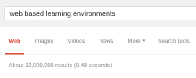
\includegraphics[]{minist-web}
    \caption{Căutare - tehnologii web}
    \label{fig:imag1}
\end{figure}

\begin{figure}[h, scale=2.0]
    \centering
    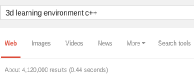
\includegraphics[]{minist-cpp}
    \caption{Căutare - tehnologii 3D și c++}
    \label{fig:imag2}
\end{figure}

\begin{table}
      \begin{center}
            \begin{tabular}{|l|l|l|}
                \hline 
                \cline{2-3}
                & $tehnologie$ & $pagini returnate$  \\ 
        	\hline
                $web$   &  32000000    &  0,48  \\
                $3D-C++$   &  4120000    &  0.44  \\
            \hline
	    \end{tabular}
        \end{center}
    \caption{Rezultate}
    \label{tab:rez}
\end{table}

\par Datele returnate de către motorul de căutare indică faptul că tehnologiile web sunt cu mult mai apreciate decât tehnologiile clasice cu grafică 3D, numărul de rezultate returnate fiind de 8 ori mai mare în favoarea tehnologiei web pentru timp de răspuns comparabil.
\chapter{Stadiul actual în domeniu}

\section{Introducere}

\textbf{ Dezvoltarea tehnologică accelerata din ultimele decenii a afectat și domeniul educației asistate de calculator. Câteva exemple de medii accesibile publicului sunt: Second Life,  Uther Academy și iSocial (http://isocial.missouri.edu/iSocial/). Fiecare dintre aceste implementări abordeaza diferit modul livrare a materialelor educative. Deși codul sursă pentru majoritatea mediilor de învățare 3D este cod proprietar, se va încerca descrierea lor din perspectiva utilizatorului în următoarele subcapitole. Secon Life este open source și poate fi studiat. Secțiunea 3.2 se azează pe similitudini în incercarea de a determina majoritatea opțiunilor pe care un utilizator le așteapta de la mediile de învățare 3D.}


\section{Abordări similare}

\par Toate exemplele notabile prezentate ulterior fac uz de avatare pentru a induce utilizatorului sentimentul de participare activă și imersiune în lumea virtuală. Utilizatorii sunt încurajați astfel sa comunice între ei atât verbal cât și prin modificarea posturii și aparenței grafice a avatarului ce îi reprezintă în lumea virtuală.
\par Aceasta tehnică este luată în considerare în implementarea aplicației descrise în acest studiu.

\section{Second Life}
\par Percepția generală este că Second Life (SL) ar fi un joc pe Internet. Nu este însă un joc organizat, cu reguli impuse și unde să fie urmărit un anumit scop. Pe situl web oficial, Second Life este descris ca fiind „o lume virtuală imaginată și creată de rezidenții ei”; într-adevăr, SL este o lume diversificată, în care poți întâlni oameni din toate colțurile lumii reale. Este o rețea de tip social, care face parte din fenomenul din Internet numit Web 2.0.

\begin{figure}[h]
    \centering
    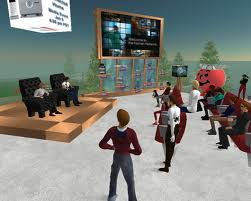
\includegraphics[]{SL}
    \caption{Eveniment în Second Life}
    \label{fig:imag3}
\end{figure}

\par Cele mai importante și interesante activități de educative sunt derulate în Second Life:
\begin{itemize}
\item Vizite asistate în muzee și teatre virtuale.
\item Cursuri în săli de clasa virtuale.
\item Jocuri de tip "orientare turistica" cu puncte intermediare și indicii cu subiect educațional.
\item Proiecte cu colaborare în echipă.
\item Cursuri online la diverse universități 
\item Panouri informative.
\item Grupuri educaționamle
\end{itemize}

\par Majoritatea facilitaților oferite de SL ar trebui să se regasească în orice platformă de e-learning cu avatare. 

\section{Uther Academy}
\par UtherAcademy este o aplicație de e-learning care facilitează participarea studenților din toata lumea la cursuri în medii imersive 3D. Liniile educative propuse sunt din categoria dezvoltarii profesionale. La data redactării acestei lucrări UtherAcademy avea deschise trei departamente :

\begin{itemize}
\item Academia de afaceri online.
\item Cursuri pentru decoratori.
\item Body arts.
\end{itemize}

\begin{figure}[h]
    \centering
    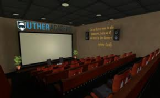
\includegraphics[]{UA}
    \caption{U.A. - aulă virtuală}
    \label{fig:imag4}
\end{figure}
    
\par Modul de prezentare generala nu diferă foarte mult de Secon Life. Studenții participa online la cursuri în clase virtuale. Procesul de învățare este supravegheat de instructori.

\section{iSocial}

\par iSocial este un mediu de învățare 3D, dezvoltat pe baza toolkit-ului pentru crearea lumilor virtuale OpenWonderland, creat pentru predarea de competențe sociale tinerilor diagnosticați cu autism (ASD). În acest scop, iSocial facilitează intracțiunea socială și oferă suport pentru dezvoltarea de competențe sociale într-un mediu sigur și complet controlat.
\par Localizarea geografica poate restricționa accesul la tratamentele și exercițiile necesare recuperării sociale a tinerilor afectați de ASD. iSocial este una dintre soluțiile rezolvării pozitive a acestei probleme.

\begin{figure}[h]
    \centering
    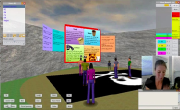
\includegraphics[]{IS}
    \caption{iSocial - panou informativ }
    \label{fig:imag5}
\end{figure}

\section{Tehnici/Tehnologii folosite}

\par Second Life (SL) este cea mai cunoscută și populară implementare a unei lumi virtuale. Deși nu este dezvoltată strict ca aplicație destinată instruirii in medii 3D, o parte însemnată a activităților desfașurate în Second Life sunt activități educcative.
\par Un studiul tehnologiilor folosite pentru dezvoltarea mediului Second Life este suficient pentru  identifica majoritatea bibliotecilor software foilosibile pentru dezvoltarea sub Linux a unei aplicații similare. S-a alcătuit o listă a tehnologiilor folosite pentru dezvoltarea SL.\ref{tab:SL_tech}
\begin{table}
      \begin{center}
            \begin{tabular}{|l|l|l|}
                \hline 
                \cline{2-3}
                $Denumire $ & $Bibliotecă/Ubuntu$ & $Utilizare$  \\ 
        	\hline
                $OpenGL$  	&  libGLU.so     	&  API pentru grfica 2D și 3D  \\
                $Zlib$   	&  libz.so     		&  Comprimare date  \\
                
                $OpenSSL$   &  libssl.so    	&  Protocoale de comunicare în rețea SSL și TLS  \\
                $OGG$   	&  libogg.so      	&  Format media audio-video  \\
                $PNG$   	&  libpng12.so      &  Imagini PNG  \\
                $GLib$   	&  libdbus-glib-1.so     &  Sistem de transmitere a mesajelor între procese  \\
                $GTK$   	&  libgtk2.0-dev 	&  GIMP toolkit  \\
                $OpenAL$   	&  libopenal-dev;libalut-dev	&  OpenAL - Biblitecă pt. redarea sunetului (audio) \\
                $Vorbis$   	&  libvorbis-dev 	&  Codec audio-video (API) \\
                $APACHE$   	&  libapr1-dev  	&  Apache portabele runtime  \\
                $JPEG$   	&  libopenjpeg.so;libjpeg.so &  Codec JPEG  \\
                $SDL$   	&  libsdl1.2-dev	&  Media Layer - faciliteaza accesul la periferice  \\
                $Boost$   	&  libboost-dev     &  Alternativa pentru C++ STL (+ comunicare în rețea) \\
                $JsonCpp$  	&  libjsoncpp-dev 	&  Interpretarea fișierelor Json (c++)  \\
            \hline
	    \end{tabular}
        \end{center}
    \caption{Tehnologii utilizabile petru dezvoltarea de medii 3D sub Linux}
    \label{tab:SL_tech}
\end{table}

\par Pentru dezvoltarea aplicației client SL se folosesc următoarele tehnologii: OpenGL pentru redarea graficii 3D, GTK pentru interfețele grafice, Boost și APACHE pentru schimbul de date în rețea între aplicația client și serverul lumii virtuale, Formatul de date JSON pentru structurarea datelor interschimbate în rețea între aplicația client și server, OpenAL pentru redarea sunetului și OGG/Vorbis ca și format/codec media și PNG/JPEG pentru redarea stocarea imaginilor. Codul sursă pentru serverul SL nu este open source.

\par O parte dintre aceste tehnologii sunt folosite pentru realizarea mediului de învățare 3D descris în această lucrare.

\chapter{Planul aplicației}
\section{Introducere}
\par \textbf{În acest capitol, în secțiunea 4.2, se stabilesc funcțiile sistemului. În secțiunea 4.3 se identifică numitorul comun al funcțiilor sistemului ca fiind facilitarea funcției de \textsf{comunicare} și se  enumeră metodele prin care comunicarea la distanță se poate implementă. După analiza punctelor slabe și a punctelor forte ale acestor metode se afirmă alegerea metodei \textsf{CLIENT-SERVER} ca fiind decizia de design de urmat și implementat. În secțiunea 4.4 se proiectează un test ca suport pentru argumentarea deciziei de design (din secțiunea 4.5).}

\section{Funcțiile sistemului}

\subsection{Minimul de funcționalitate \\ de cercetat și implementat}
\par Prin analiza funcțională, bazata pe observație liberă a câtorva dintre mediile 3D existente și accesibile pe internet, am putut determina  o parte din funcțiile absolut necesare ale sistemului.
\par Aceste funcții sunt parte integrantă a cerințelor sistemului. La acestea se mai adaugă cerințele de ordin general precum: implementarea unei interfețe grafice ușor de folosit, mentenabilitatea și extensivitatea sistemului, etc.. \\
\par \textbf{Funcții ale sistemului:}
\begin{itemize}
\item Utilizatorii sistemului sunt conștienți de prezența altor utilizatori (persoane reale) în lumea virtuală. Sistemul îndeplinește funcția de liant prin facilitarea schimbului de idei între utiliztori.
\item Utilizatorii pot interacționa cu o parte dintre obiectele din umea virtuală. În unele situații, rezultatul acestei interacțiuni conduce la modificări permanente în reprezentarea lumii virtuale simulate. Sistemul îndeplinește funcția de stocare a modelului tridimensional al lumii viruale, inclusiv a starii acestui model, stare ce poate fi modificată de către utilizatori.
\item Sistemul va stoca informațiile referitoare la identificarea utilizatorilor. Această identificare nu presupune stabilirea identității persoanei reale ci are funcția de a servi ca identificator pentru un catalog al progresului utilizatorului în procesul de învățare.
\item Utilizatorii vor putea contribui la extinderea lumii virtuale prin publicarea de materiale educative dezvoltate de cătrea aceștia. Sistemul va permite contribuția utilizatorilor va avea funcția de stocare și prezentare a noilor materiale educative.
\end{itemize}

\par Cea mai mare parte dintre aceste funcții se vor implementa în aplicația software demonstrativă atașată acestui proiect.

\subsection{Funcționalitate extinsă}

\par Următoarele funcții nu vor fi incluse in software-ul demonstrtiv, dar sunt recunoscute ca necesare pentru orice sistem de învățare.

\begin{itemize}
\item Funcția de asigurare a accesibilității pentru persoanele cu deficiențe de vedere sau deficiențe motorii.
\item Funcția de redare a tuturor formelor de conținut media. Din motive tehnice și pentru complexității aplicației demonstrative, în mare măsură se vor exclude conținuturile media video și audio.
\end{itemize}

\section{Decizie privind design-ul sistemului}

\par Toate funcțiile primare ale sistemului fac referire la facilitarea comunicării între utiliztori pentru asigurarea schimbului liber de informații, sau între sistem și utilizatori cu scopul stocării și/sau accesării de date cu pentru diverse scopuri legate de funcționarea sistemului sau menținerea unui catalog al progresului utilizatorilor. Aceste schimburi de date se fac la distanță, pentru a nu condiționa geografic participarea la procesul de învățare.
\par Pentru implementarea comunicării în rețea se va alege unul dintre cele două modele general utilizate în practică: modelul client-server \ref{fig:imag5} și modelul p2p (point to point) \ref{fig:imag4}.

\par \textbf{Modelul P2P} este un model descentralizat în care fiecare nod este atât client cât și server pentru celelalte noduri din rețea. Modelul este mai dificil de implementat, consistența datelor în rețea este mai greu de menținut și administrarea este destul de dificilă. Deși modelul este mai robust prin faptul că piederea unui nod din rețea nu conduce la sistarea serviciului deoarece funcția de server este preluată de restul nodurilor; acest model nu este cel mai bun pentru implementarea unei lumi virtuale, unde consistența datelor este foarte importantă. Aceasta consistență a datelor permite tuturor utilizatorilor să perceapă aceeași lume virtuală. 

\begin{figure}[h]
    \centering
    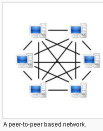
\includegraphics[]{p2p_2}
    \caption{Modelul P2P}
    \label{fig:imag4}
\end{figure}

\textbf{Modelul Client-Server} este un model centralizat în care fiecare nod client comunică și depinde de serviciile nodului server. Acest model este relativ ușor de implementat, ușor de administrat, consistența datelor poate fi verificată și inpusă la nivelul serverului și stocarea datelor poate fi facută centralizat la același nivel. Cel mai mare dezavantaj al acestui model este faptul că, pierderea accesului la server prin oprirea acestuia face tot sistemul inoperabil. Acest model este mult mai portivit pentru implementarea unei lumi virtuale și a unui mediu de învățare 3D. 

\begin{figure}[h]
    \centering
    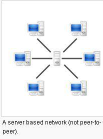
\includegraphics[]{serverbased_2}
    \caption{Modelul Client-Server}
    \label{fig:imag5}
\end{figure}

\section{Teste}
\par Testul constă în simularea comunicării dinspre server către client. Un server va incerca să timită mesaje către un număr de 20 aplicații client care salveaza în câte un fișier mesajele primite de la server. Mesajele vor avea o lungime cuprinsă între 10 și 1024 caractere.
\par Se consideră testul reușit dacă toate mesajele ajung la toate aplicațiile client în aceeași ordine și într-un timp copmarabil (sub 1 secundă distanță).
\par Pentru rularea testului se codifică două aplicații demonstrative.

\section{Argumentarea deciziei \\ pe baza rezultatelor testării}

\par Testul a fost executat cu succes. Datele obținute se află în ANEXA A.
\par Deoarece comunicarea între aplicațiile client și server sunt livrate consistent și la timp, se concluzionează faptul că se poate folosi schema client-server pentu implementarea aplicației.

\chapter{Design-ul aplicației server}
\section{Introducere}
\par \textbf{În acest capitol, în secțiunea 5.2, se stabilesc funcțiile serverului și se prezintă tehnologiile folosite la producerea aplicației server. În secțiunea 5.3 se explică mecanismul adoptat pentru atingerea unui scop important, ”scalabilitatea aplicației” . În secțiunea 5.4 se stabilește modul și formatul de reprezentare a datelor transmise între aplicația client și aplicația server. Secțiunea 5.5 este dedicată prezentării părții celei mai relevante din diagrama claselor. În secțiunea 5.6 sunt stabiliți parametrii testului privind scalabilitatea aplicației, codificarea testului și rezultatele fiind expuse în Anexa B. Testul modului de comunicare și a eficienței comunicării intre client și server s-a efectuat pentru capitolul anterior, rezutatele fiind publicate în Anexa A. } 

\section{Funcțiile aplicației server}
\subsection{Funcții de bază ale serverului} 
\begin{itemize}
\item Asigurarea comunicării înspre una sau mai mule aplicații client.
\item Asigurarea comunicării între clienți prin intermediul serverului.
\item Stocarea datelor referitoare la activitățile întreprinse de către utilizatori într-o bază de date.
\item Eliberarea datelor din baza de date, la cererea utilizatorului.
\item Stocarea și publicarea informațiilor ce descriu geometria lumii virtuale.
\item Stocarea și publicarea acțiunilor utilizatorilor ce au efect asupra limii virtuale.
\end{itemize}

\par Serverul are scop demonstrativ. Funcția de securitate a datelor la transfer și la stocare este ignorată. De asemenea, implementarea funcțiilor se realizează in cel mai simplu mod posibil, pentru reducerea complexității și dimensiunii aplicației.

\subsection{Aspecte tehnice și principii generale de design}
\subsubsection{Limbaje de programare}
\par Codificarea aplicției server se va executa în limbajele de programare Java și JavaScript.
\par Java este probabil cel mai potrivit limbaj pentru implementarea aplicațiilor server datorită numărului mare de  biblioteci software utilizate pentru realizarea schimbului de date în rețelele de calculatoare. Acestea pun la dispoziția programatorului o multitudine de funcții de nivel înalt pentru comunicarea la distanță folosind diverse protocoale de comunicație de nivel înalt (HTTP/FTP/SSH/etc), cât și funncții de nivel mediu (bazate pe protocoalele TCP/UDP/etc..). Implementarea unei aplicații scalabile prin utilizarea ”plug-in”-urlior este relativ usor de realizat. Existența unui interpretor JavaScript pentru platforma Java este încă un argument în favoarea folosirii acestui limbaj de programare.
\subsubsection {Sistemul de operare}
\par Aplicațiile java sunt extrem de portabile, acestea rulând pe virtual orice sistem de operare și pe orice platformă hardware. Serverul mediului de învățare 3D va rula în varianta pentru GNU/Linux a ”Mașinii Virtuale Java” (JVM). Fiabilitatea kernelului sistemului de operare Linux va afecta pozitiv viteza de rulare a mașinii virtuale java cu efect direct asupra performanței aplicației server dezvoltate pentru mediul virtual 3D.
\subsubsection{Principii generale de design}
\par \textbf{Pentru intermedierea comunicării între utilizatori} sau pentru orice fel de notificări trimise utilizatorilor s-a ales un tipar cunoscut în domeniul informatic sub numele ”Observer Pattern”. Această metodă definește și utilizează o dependență 1 → n între obiecte astfel încât un obiect își modifică starea, toate obiectele dependente sunt notificate. Aplicat, în cazul serverului (1) , când un set de date este prelucrat, utilizatorii (n) sunt notificați.
\par \textbf{Pentru a realiza o aplicație scalabilă} se utilizează mecanismul de extindere dinamică a fincționalității cu ”plug-in”-uri. 
\section{Mecanism pentru obținera \\ scalabilității aplicației server}

\par Se va urmări o cît mai mare flexibilizare a sistemului, astfel încât dezvoltarea ulterioară sa fie cât mai facilă. Pentru realizarea acestui obiectiv se va urmări integrarea limbajului de scriptare JavaScript, în serverul sistemului. Se are în vedere folosirea mecanismului de extindere dinamică a funcționalității sistemului prin ”plug-in”-uri. 
\par Utilizatorul, prin intermediul programului client al mediului virtual 3D, expediază \textbf{comenzi} și \textbf{informații} către server cu \textbf{scopul} de a fi prelucrate de către server și returnate sub forma de comezi ce urmează a fi executate de către aplicația client, cu \textbf{efecte} asupra reprezentării mediului virtual 3D.

\begin{center}
\rule{150mm}{.1pt}
\end{center}

\par \textbf{DEF:} \textit{Un} \textbf{plug-in} \ref{fig:imag35} \textit{este o componentă software care poate fi integrată de către aplicația gazdă la momentul execuției sau imediat la începutul procesului de execuție. De cele mai multe ori ”plug-in”-urile sunt salvate în formă binară.}

\begin{figure}[h]
    \centering
    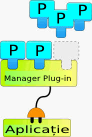
\includegraphics[]{PLA}
    \caption{Arhitectura Plug-in}
    \label{fig:imag35}
\end{figure}

\begin{center}
\rule{150mm}{.1pt}
\end{center}

\subsection{Interfața PLUG-IN-ului}
\par ”Plug-in”-urile aplicației server implementează următoarea interfață:
\begin{verbatim}
public interface CommandTypeDependentInterpreter {
      
      public static final int XML_FORMAT = 1;
      public static final int PALIN_TEXT_FORMAT = 2;
      public void prepareResponse(ServerCommand execCmd, int format);
      String getInterpretedResult();

}
\end{verbatim}

Un plug-in extinde funcționalitatea aplicației server prin introducerea unei noi modalități prin care serverul răspunde la o cerere din partea aplicației client. În prima etapă, plug-in-ul preia comanda expediată de aplicația client prin intermediul metodei: \begin{center} \textit{-- prepareResponse(ServerCommand execCmd, int format) --}
\end{center} În a doua etapă, rezultatul interpretării și procesării datelor de către plug-in se va returna în vederea expedierii către utilizator.

\subsection{Tipuri de plug-in-uri dezvoltate pentru serverul mediului de învățare 3D}
\par Două \textbf{tipuri de plug-in-uri} au fost dezvoltate pentru aplicația server. Primul tip de plug-in este \textbf{”clasic”}, implementat folosind 100\% limbajul Java. Al doilea tip de plug-in este \textbf{”hibrid”}. La inplementarea acestuia sunt utilizate două libmaje de programare: \textbf{Java și JavaScript}. Aces tip de plug-in este o noutate.

\par În principiu, un plug-in hibrid are rolul de a executa la nivelul serverului instrucțiuni codificate în limbaj JavaScript în numele aplicației client. Rezultatele sunt încapsulate în format XML și sunt returnate programului client pentru interpretere. Executarea comenzilor primite de la aplicația client este precedată de următorii doi pași pregătitori: inițializarea unui motor de prelucrare JavaScript ( clasa ScriptEngineManager ) și concatenera la comanda utilizatorului a unei biblioteci care conține obiecte JavaScript utile.

\par \textbf{Funcționarea plug-in-ului hibrid }


\par Avantajele plug-in-urilor hibride:
\begin{itemize}
\item 
\item
\item
\end{itemize}

\par Dezavantajele plug-in-urilor hibride:
\begin{itemize}
\item 
\item
\end{itemize}


\subsection{Descrierea mecanismului de încărcare a plug-in-urilor}

\chapter{Design-ul aplicației client}
\section{Introducere}
\par \textbf{În acest capitol, în secțiunea 6.2, se stabilesc funcțiile aplicației client. În secțiunea 6.3 se prezintă conceptul aplicației software și se enumeră tehnologiile folosite la realizarea acestuia în structura următoare: }

\begin{itemize}
\item 6.3.1 - Cercetare a modului de livrare a conținutului educativ în mediul 3D.
\item 6.3.2 - Tehnologii utilizate pentru redarea 3D a lumii virtuale.
\item 6.3.3 - Tehnologii utilizate pentru relizarea interfaței grafice (GUI).
\item 6.3.4 - Tehnologia utilizată pentru comunicarea cu serverul.
\end{itemize}

\par \textbf{ În secțiunea 6.4 se explică mecanismul adoptat pentru atingerea unui scop important, ”scalabilitatea aplicației” . În secțiunea 6.5 se explică mecanismul CERERE-PROCESARE-RASPUNS. În aceeași secțiune se prezintă formatul de reprezentare a datelor transmise între aplicația client și aplicația server. Secțiunea 6.6 este dedicată prezentării diagramei claselor. În secțiunea 6.7 se enunță parametrii testării aplicației client. Rezultatele acestei testări expuse în același capitol. } 

\newpage

\section{Funcțiile aplicației client.}

\par Aplicația client are scop demonstrativ. Implementarea se va executa în cel mai simplu mod posibil, cu interfețe utilizator minimale. Funcțiile de bază ale aplicației client sunt enumerate dar implementarea nu se execută în integralitate.

\textbf{Funcții de bază:}
\begin{itemize}
\item Redarea 3D a obiectelor lumii virtuale.
\item Schimbul de date între aplicație și server, după modelul CERERE - RĂSPUNS.
\item Facilitarea comunicării directe între participanții la procesul de învățare în mediul virtual.
\item Reprezentarea utilizatorilor în mediul virtual prin intermediul avatarelor. Fiecare utilizator va fi reprezentat de un avatar identificabil de către ceilați utilizatori.
\item Facilitarea cooperării între utilizatori.
\item Aplicația, în anumite instanțe, va asista utilizatorul în procesul de învățare. 
\end{itemize}

\section{Conceptul aplicației și tehnologiile utilizate.}

\par Interfața aplicției cu utilizatorul este esențială pentru asugurarea unei experințe cât mai plăcute în timpul utilizării. Pentru realizarea interfețelor se vor respecta următoarele aspecte: simplitate, etichete și denumiri sugestive.
\par Designul interfeței grafice 2D este minimal. Se va dezvolta în principal componenta de redarea 3D a obiectelor din mediul virtual.

\begin{figure}[ht]
    \centering
    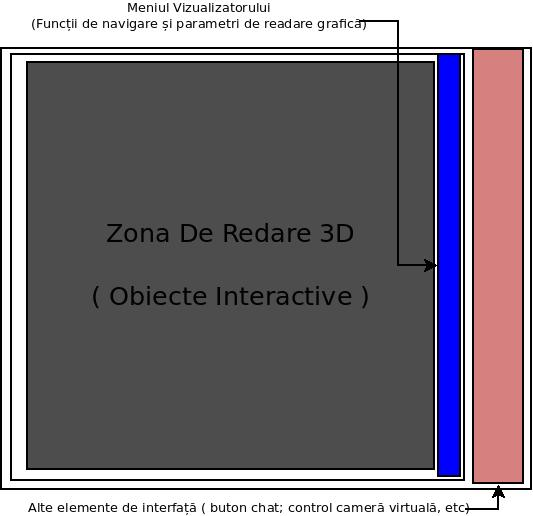
\includegraphics[scale=0.32]{concept}
    \caption{Dispunerea elementelor în interfața grafică}
    \label{fig:vorldd}
\end{figure}

\newpage
\subsection{Modul de livrare a conținutului educativ în mediul 3D}

\begin{figure}[ht]
    \centering
    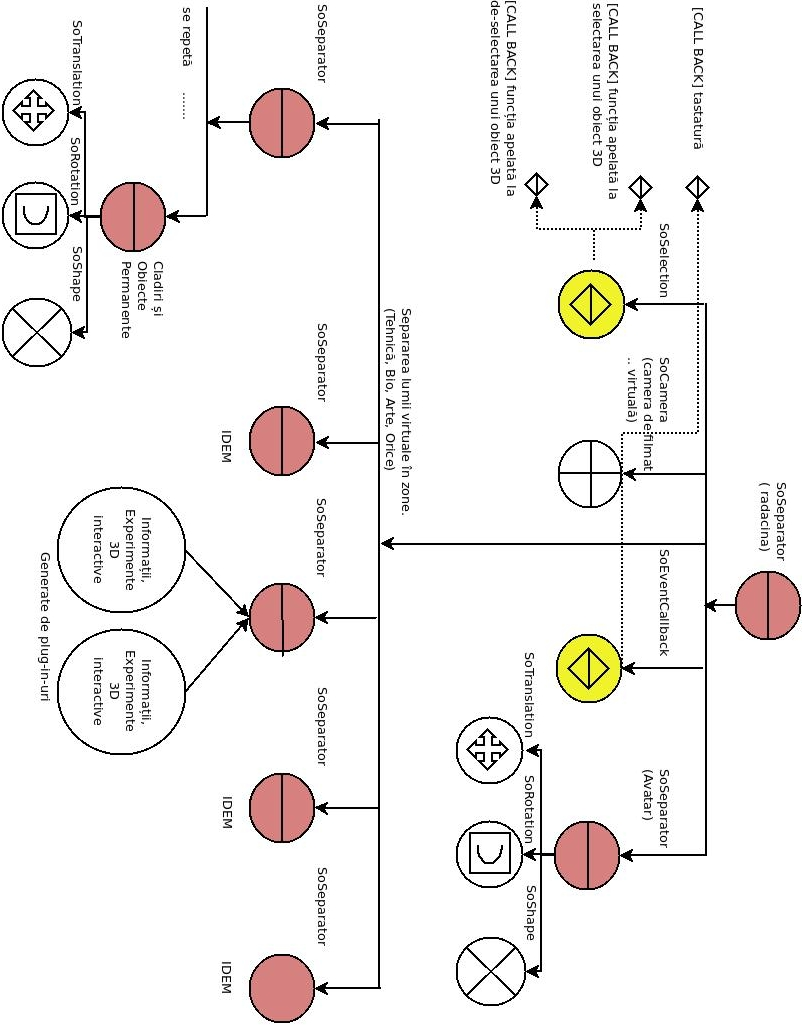
\includegraphics[scale=0.4]{WRLD}
    \caption{Mediul 3D și materialul educativ interactiv}
    \label{fig:vorldd}
\end{figure}

\newpage

\subsection{Tehnologii utilizate pentru redarea 3D a mediului de învățare.}
\subsubsection{Sistemul de operare}
\par Sistemul de operare ales pentru dezvoltarea aplicatiei este GNU/Linux (sitemul de operare GNU + kernelul Linux), distribuția Ubuntu, un sistem de operare modern, foarte asemanător sistemului de operare Unix, dezvoltat de către comunitățile “Free Foftware” și “Open Source”.
\par Motivele alegerii acestui sistem de operare sunt urmatoarele: 
\begin{itemize}
\item Stabilitatea sistemului de operare. 
\item Performanța sistemului de operare. 
\item Simplitatea în instalare și menținere.  
\item Multitasking și managementul memoriei foarte eficient implementate.
\item Compilatoarele, librariile grafice și cele mai importante instrumente pentru dezvoltarea de medii 3D sunt ușor de instalat șconfigurat, sunt gratuite și bine documentate pentru GNU/Linux.
\end{itemize}

\subsubsection{Limbajul de programare}

\par Limbajul de programare ales pentru realizarea aplicației client este C++. Sunt motivat în alegerea mea de urmatoarele caracteristici ale acestui limbaj:  
\begin{itemize}
\item Aplicațiile programate în C++ ruleaza vizibil mai rapid decat aplicațiile realizate în alte limbaje de programare.
\item O multitudine de biblioteci software utile sunt implementate în C++.
\item Aplicația finală poate fi compilată pentru mai multe platforme.
\item C++ este limbajul de programare preferat de dezvoltatorii aplicatii bazate pe grafica 3D.
\end{itemize}
     
\par Compilatorul ales este g++ din colectia GCC (Gnu Compilers Collection). 

\subsubsection{Limbje și biblioteci software utilizate \\ pentru reprezentarea mediului virtual 3D}

\par Când se alege o bibliotecă 3D, factorii care trebuiesc luaţi în considerare sunt: performanța,
existența şi calitatea documentaţiei, platformele care acceptă biblioteca grafică 3D, existenţa unui
format standardizat pentru a descrie obiectele grafice şi interacţiunile obiect, licenţiere etc. Ţinând cont de criteriile menţionate mai sus s-a ales biblioteca Coin3D cu suport VRML (Virtual Reality Modeling
Language). 

\subsubsection{Coin 3D (Open Inventor reimplementat cu suport pentru V.R.M.L.)}
\par \textbf{Generalități}
\par Coin se bazează pe librăria grafică 3D OpenGL (The Open Graphics Library), și își are rădăcinile în Open Inventor 2.1 API, cu care Coin este încă compatibil. Precursorul bibliotecii Coin3D, Open Inventor, își bazează modul de păstrare și manipularea a obiectelor grafice, pe libraria și structura claselor C++ original proiectată pentru SGI.\cite{COIN_COMM}
\par Open Inventor a devenit repede după lansare biblioteca grafică standard de facto pentru vizualizare 3D și software de simulare vizuală în comunitatea științifică și inginerească, și mai târziu, bază pentru formatul standard VRML1. 
\par Există multe publicații pe subiectul Open Inventor, cele mai importante fiind: “The Inventor Mentor”, “The Inventor Toolmaker”, amandouă fiind recomandate pentru cei ce doresc să învețe sa utilizeze Open Inventor. Aceleași materiale de studiu se pot folosi pentru inițierea în utilizarea librariei grafice Coin3D.\cite{COIN_COMM}
\par Coin3D a fost dezvoltată independent, de la zero înainte ca Open Inventor să devină open source. Coin și-a atins țelul compatibilității cu standardul Open Invetor 2.1 în toamna anului 2000 și de atunci a fost și-a dezvoltat foarte mult numarul de caracteristici, variind de la suportul pentru sunetul 3D (deficitar pentru sistemul de operare GNU/Linux) la suportul GLSL shader, formate de fișiere suplimentare cum ar fi VRML97, și un numar larg de schimbări interne pentru a ține pasul cu noul OpenGL, optimizat cu o varietate mare de tehnici ce nu erau disponibile la început.\cite{COIN_COMM} 
\par \textbf{Istoric}
\par Coin își are începuturile în anul 1995, fiind conceput ca o librarie de redare grafică pentru standardul VRML 1.0 . Initial a fost dezvoltată plecând de la librăria Qv a SGI care are rolul de a analiza fisierele în format VRML 1.0. După ani de extindere anevoioasă a bibliotecii soft, începând cu noi funcționalități de redare și exportare precum VRML 1 și VRML 2, în anul 1997 s-a ajuns la o reală nevoie de reproiectatare.\cite{COIN_COMM}
\par La prima vedere API-ul are o asemănare izbitoare cu Open Inventor. Conceptele utilizate de către Open Inventor sunt deseori amintite ca o bună metodologie de proiectare în multe cărti de inginerie software, astfel că o parte dintre programatorii care s-au ocupat de dezvoltarea acestuia și care aveau deja experiența cu această librarie, au luat conceptul Open Inventor ca un exemplu demn de urmat. Concomitent cu identificarea strategiei de rescriere a codului, s-a luat decizia de colaborare cu membrii comunității Free Software care au contribuit cu o serie de idei tehnice interesante. Ca o urmare firească a acestei colaborări, libraria s-a dezvoltat ca o alternativă liberă la varianta Open Inventor, cu suport pentru sistemele de operare GNU/Linux, IRIX, Windows, Cygwin și Mac OS X.\cite{COIN_COMM}

\subsubsection{V.R.M.L. (Virtual Reality Modeling Language)}
\par VRML este un limbaj de modelare a lumilor virtuale și un standard internațional pentru descrierea formelor și a scenelor pentru World Wide Web. Organizația responsabilă cu dezvoltarea și publicarea standardului VRML este ”Web 3D Consortium” anterior cunoscută sun numele ”VRML Consortium”. În prezent standardul a ajuns la versiunea a doua.
\par În principiu, o lume virtuală descrisă cu limbajul VRML se poate reprezenta printr-o structură arborescentă în care „nodurile și frunzele” arborelui sunt noduri VRML. \cite{VRML}

\begin{figure}[h]
    \centering
    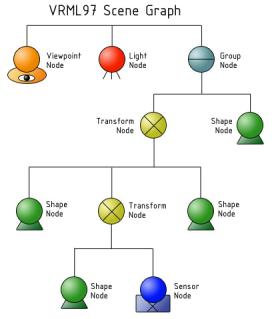
\includegraphics[scale=1.1]{vrml-scene-graph}
    \caption{Graf VRML (exemplu)}
    \label{fig:graphvrml}
\end{figure}

\par Modul în care lumea virtuală este afișată pe display-ul computerului  este influențat de ordinea și amplasarea nodurilor în arbore. Fiecare nod este redat în mod grafic după următoarele reguli:\cite{NADEAU} \cite{NADEAU2}

\begin{itemize}
\item Redarea unui grup de noduri se face în ordine, de regulă, de la stânga la dreapta. Aplicând această regulă la ilustrația precedentă \ref{fig:graphvrml}, putem trage concluzia că nodurile de tip ”transformări” (transform) au efect asupra nodului ”Formă geometrică” (Shape Node) doar dacă sunt amplasate înaintea acestuia.
\item Fiecare nod execută propria afișare și afectează starea următoarelor noduri prin modificarea proprietăților membre. Spre exemplu, un obiect al carui suprafață este reflexivă sau radiantă din puntul de vedere al luminozității, poate afecta modul în care urmatoarele noduri sunt iluminate.
\item Nodurile de tip ”transformare” (Transform Node) se influențează prin combinare (ex: două rotații de 90$^{\circ}$ se acumulează formând o rotație de 180$^{\circ}$ ).
\item Nodurile de tip ”formă geometrică” sunt afișate în modul dictat de starea actuală (ultima culoare setată, ultima luminozitate setată).
\item Nodurile de tip SoSeparator (separatoare), spre diferență de SoGroup (grup), salvează starea actuală înainte de a-i parcurge și afișa nodurile membre. Această stare este restaurată după parcurgerea separatorului. Astfel, nodurile din separator nu afectează nodurile următoare, fiind izolate.
\item Nodurile sunt ”construite” la punctul de coordonate XYZ = (0,0,0) dacă nu sunt afectate de nici o transformare.
\item Sistemul de coordonate VRML este următorul : pentru valori pozitive, axa Y este orientată în sus, axa X este orientată spre dreapta și axa Z este perpendiculară pe axele XY și este orientată spre observator. \ref{fig:vrmlaxes}
\item Pentru efectuarea rotațiilor se aplică regula mâinii drepte. Sensul pozitiv al rotației este sensul invers acelor de ceasornic. Rotația se exprimă în grade radian. \ref{fig:vrmlrot}
\end{itemize} 

\begin{figure}[h]
    \centering
    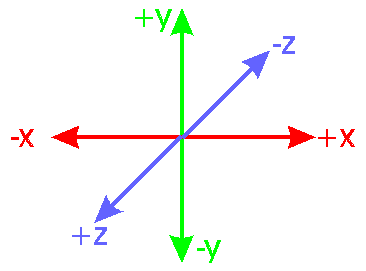
\includegraphics[scale=0.5]{vrmlaxis}
    \caption{Axe}
    \label{fig:vrmlaxes}
\end{figure}

\begin{figure}[h]
    \centering
    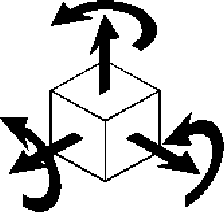
\includegraphics[scale=0.5]{rotation-rule}
    \caption{Rotație}
    \label{fig:vrmlrot}
\end{figure}

\par \textbf{Animații descrise în VRML}
\par Scenele 3D descrise cu ajutorul limbajului VRML pot fi animate și pot fi programate să răspundă la comenzile utilizatorului. Acestă interacțiune se poate realiza în două moduri: programatic, prin accesarea și modificarea nodurilor grafului scenei VRML prin rutinele unui program dezvoltat de utilizator (în C++/Python/etc); sau prin folosirea mecanismulor de descriere a interacțiunilor și animațiilor pus la dispoziție de limbajul VRML.
\par Interactivitatea în VRML se realizează prin transmiterea de valori ale ”proprietăților” între diversele noduri ale grafului VRML. Când un nod trimite informații către un alt nod, se crează un \textbf{eveniment (”event”)}, o structură ce transportă două informații date (valori) și informație referitoare le timp (timestamp) pentru exprimarea momentului în care evenimentul s-a produs, cu scopul asigurării integrității logice pentru secvențele de evenimente [CITE COMENT Rohel]. Mecanismul animației presupune crearea unei conexiuni explicite între noduri cu ajutorul construcției sintactice \textbf{ROUTE} între ”câmpurile” ce stochează atributele nodurilor implicate în animație. Majoritatea nodurilor sunt construite după structura:
\begin{verbatim}
nod { 
   camp             (field)         ; inaccesibil
   eveniment primit (eventIn)       ; permite doar scriere
   eveniment emis   (eventOut)      ; permitere doar citire
   câmp expus       (exposedField)  ; permite citire și srcirere
}
\end{verbatim} 
Evenimentele transmise prin câmpul eventOut al unui nod, vor putea fi recepționate de un al doilea nod prin câmpul eventIn, având ca efect animația nodului receptor.	\ref{fig:vrmlanim}	

\begin{figure}[h]
    \centering
    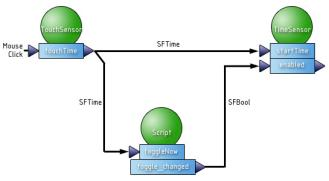
\includegraphics[scale=1.5]{vrml-anim}
    \caption{ANIMAȚIE VRML}
    \label{fig:vrmlanim}
\end{figure}
% Roehl, B., et al. (1997), Late Night VRML 2.0 with Java. Emeryville: Ziff-Davis.
\newpage
\par Exemplu: (Orientarea obiectului grafic se modifică în timp, din momentul activării senzorului de atingere)
\begin{verbatim}
# VRML V2.0 utf8 

DEF Touch TouchSensor { } 
DEF Timer1 TimeSensor { } 
DEF Rot1 OrientationInterpolator { } 

DEF Frame1 Transform { 
	children [ 
		Box { }   
		] 
} 

ROUTE Touch.touchTime TO Timer1.set_startTime 
ROUTE Timer1.fraction_changed TO Rot1.set_fraction 
ROUTE Rot1.value_changed TO Frame1.set_rotation

\end{verbatim}

\subsection{Tehnologii utilizate pentru relizarea interfaței grafice (GUI)}
\par Interfețele grafice se vor implemeta folosind atât bibilotecile software Qt/SoQt cât și tehnologii Web/HTML. Interfețele Web sunt adoptate deoarece implementarea lor necesită mai puțin timp și sunt mult mai dinamice decât interfețele implemetate în c++ utilizând bibliotecile Qt/SoQt.

\subsubsection{Qt}

\par Qt este un cadru software pentru programarea aplicațiilor multi-platformă și pentru dezvoltarea de interfețe grafice folosind  ca limbaje: C++, QML, CSS și JavaScript. Librariile Qt și uneletele de dezvoltare sunt eliberate prin licențe compatibile cu modelul ”open source”. 
\par Qt implementează metode inteligente pentru realizarea comunicării între divesrele obiecte ale interfeței grafice. Metoda constă în conectarea evenimentelor prelute de elementele de interfță la rutinele asociate cu aceste evenimente sau conectarea la alte evenimente. Acest lucru se realizează automat, cu ajutorul unui meta-compilator care generează codul necesar conectarii evenimentelor (SIGNAL) la rutine (SLOT). \ref{fig:sig-slot} \cite{QT}

\begin{figure}[h]
    \centering
    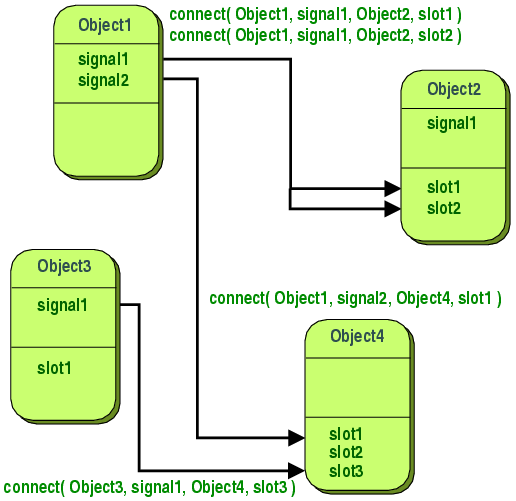
\includegraphics[scale=0.5]{qtconn}
    \caption{Mecanismul SIGNAL-SLOT}
    \label{fig:sig-slot}
\end{figure}

\newpage
\subsubsection{SoQt}
\par SoQt furnizează programatorului o interfață de nivel înalt în C++. Librăria, include o ierarhie de clase cu rol de componentă de vizualizare (viewers), cu funcționalități diferite, împreună cu o serie de modalități de control a interacțiunii dintre camerele virtuale de filmat și scena 3D. SoQt este practic liantul dintre librăriile de interfețe Qt și Coin 3D.
\subsubsection{Interfețe Web/HTML prin mecanismul ”QtWebKit Bridge”}
\par Mecanismul ”WebKit bridge” este parte a bibliotecii sotware Qt. Prin acest mecanism se facilitează accesul obiectelor codificate in JavaScript la rutinele codificate în c++ în aplicația realizată cu ajutorul bibliotecii software Qt. În acest fel, o pagină web poate fi programată ca o interfață pentru un program codificat în c++. \cite{QT} 

\subsection{Tehnologia utilizată pentru comunicarea cu serverul}

\par Viteza de execuție a aplicațiilor codificate în C++ și existența librariei Coin3D, este motivul alegerii acestui limbaj pentru implementarea aplicației client. Ultimul standard adoptat de ISO include extensii pentru limbaj și adaugarea de module noi la librăria standard. Cea mai binevenită modificare este suportul pentru programarea firelor de execuție în modelul tehnicii OOP. 
\par Pentru programarea rețelelor de calculatoare nu există suport modern, acest aspect fiind în agenda ISO pentru următorul standard. Pentru acest ”task” am folosit librăria Boost Asio, o subcomponentă a biblotecii software Boost. 
\par Boost Asio implemetează un model modern bazat pe modelul OOP, pentru programarea asincronă a operațiilor I/O la nivel scăzut și programarea aplicațiilor pentru rețele de calculatoare (cu asincronism în ce privește trimiterea/primirea de date în rețea). \ref{fig:asio}

\begin{figure}[h]
    \centering
    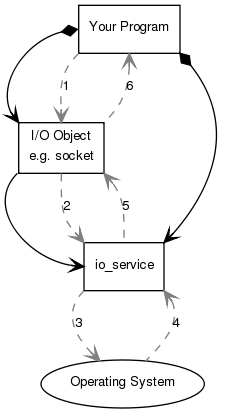
\includegraphics[]{sync_op}
    \caption{Mecanismul I/O asincron}
    \label{fig:asio}
\end{figure}

\section{Decizie privind design-ul aplicației client.}
\par Se va urmări o cît mai mare flexibilizare a sistemului, astfel încât dezvoltarea ulterioară sa fie cât mai facilă. Se are în vedere folosirea mecanismului de extindere dinamică a funcționalității sistemului prin ”plug-in”-uri. 	Plugin-urile vor putea fi descărcate din surse externe în timpul rulării aplicației client, și incluse dinamic în aplicație, fără a se întrerupe rularea programului. Un plug-in va prelua funcția de încărcare de cursuri interactive și activități educative diverse. 

	 Un plug-in respectă următoarea interfață:
\begin{verbatim}
#ifndef L3DCLIENT_PLUGIN_H
#define L3DCLIENT_PLUGIN_H

#include <Inventor/nodes/SoSeparator.h>
#include <string>
 
  //interfața plug-in
  extern "C" void get_plug_in( std::string data, SoSeparator* insertionPoint );
  //pointer la o funcție cu aceeiași parametri și tip returnat ca plug-in-ul
  typedef void (*PLUG_IN)( std::string , SoSeparator*);

#endif
\end{verbatim}	
	
\par Plug-inurie sunt în fapt funcții standardizate, compilate în librării dinamice ”Shared Object”. Descărcarea librăriilor de pe internet se va realiza prin apelarea comenzii Linux wget. 
\par Compilarea bibliotecilor software dinamice se efectuează cu specificarea unor parametri speciali pentru compilator. \cite{DYN_LIBS}
\begin{itemize}
\item \textbf{-Wall}, afișează toate mesajele de alarmă
\item \textbf{-fPIC}, ”Position independent code”; pubctul de încărcare a instrucțiunilor variază la bibliotecile dinamice. 
\item \textbf{-c}, doar compilare 
\item \textbf{-Wl,-snoname,<name>}, instrucțiuni către link-editor pentru a genera obiecte dinamice
\end{itemize}
Următorul script crează biblioteci software dinamice ce pot utiliza clase Qt, Boost și Coin:
\begin{verbatim}
#!/bin/bash
# ->  mod de foflosire: 
# $>  build_lib.sh <sursa.cpp> <denumire fisier obiect> <nume biblioteca>
# ->  DOAR sursei .CPP i se adauga extensia !!!!!!!!!!!!!!!!!!!!!!!!!!!!! 

CPPFLAGS_COIN=`soqt-config --cppflags`
CXXFLAGS_COIN=`soqt-config --cxxflags`
LDFLAGS_COIN=`soqt-config --ldflags`
LIBS_COIN=`soqt-config --libs`

CPPFLAGS_QT=`soqt-config --cppflags`
CXXFLAGS_QT=`soqt-config --cxxflags`
LDFLAGS_QT=`soqt-config --ldflags`
LIBS_QT=`soqt-config --libs`
INCLUDEDIR_QT=" -I/usr/include/qt4 -I/usr/include/qt4/QtCore \
                -I/usr/include/qt4/QtGui -I/usr/include/qt4/QtOpenGL \
                -I/usr/include/qt4/QtWebKit "

BOOST_CPPFLAGS=" -pthread " 
BOOST_FILESYSTEM_LDFLAGS=" -L/usr/local/lib -Wl,-R,/usr/local/lib "
BOOST_FILESYSTEM_LIBS=" -lboost_filesystem "
BOOST_SYSTEM_LDFLAGS=" -L/usr/local/lib -Wl,-R,/usr/local/lib "
BOOST_SYSTEM_LIBS=" -lboost_system "
BOOST_THREAD_LDFLAGS=" -L/usr/local/lib -Wl,-R,/usr/local/lib "
BOOST_THREAD_LIBS=" -lboost_thread -lboost_system -pthread "

#
# [ -Wall ] display all warnings
# [ -fPIC ] generate Position Independent Code
#
#  MODEL g++ -c -Wall -fPIC plugin1.cpp  -o plugin1.o

g++ -std=c++11 -c -Wall -fPIC $INCLUDEDIR_QT $1 -o $2.o 

#
# [ -Wl,-snoname,<name> ] instuct the linker the
# linker to generate a Dynamic Shared Objects
# instead of an application
#
g++ -std=c++11 $BOOST_CPPFLAGS $CPPFLAGS_COIN $CXXFLAGS_COIN $CPPFLAGS_QT  \
     $CXXFLAGS_QT -I$INCLUDEDIR_QT -shared -Wl,-soname,$3.so -o $3.so $2.o \
     $BOOST_SYSTEM_LDFLAGS $BOOST_SYSTEM_LIBS $BOOST_THREAD_LIBS  \
     $BOOST_THREAD_LDFLAGS $BOOST_FILESYSTEM_LDFLAGS $BOOST_FILESYSTEM_LIBS \
     $LDFLAGS_COIN $LIBS_COIN  $LDFLAGS_QT $LIBS_QT
	
\end{verbatim}
\newpage
\par \textbf{Exemplu de implementare a unui plug-in}
\par Exemplul listat este plug-in-ul care are rolul de a crea si anima avatarele celorlalți utilizatori. Acestea își schimbă orientarea și poziția în spațiu la fiecare 0.5 secunde. Parametrii furnizați de aplicație plug-in-ului reprzintă:

\begin{itemize}
\item Un număr variabil de informații și parametri primiți de la server, în format XML, reprezentînd numele acțiunii ed executat la nivelul aplicației client și datele necesare pentru implemetarea acestei acțiuni.
\item Un pointer spre un ”separator” al lumii virtuale, reprezentând zona în care programatorul plug-in-ului poate insera grafica 3D dorită.
\end{itemize}

\begin{verbatim}
#include "../src/plugin.h"
#include "../src/vrml_utils.h"
#include <Inventor/nodes/SoSeparator.h>
#include <Inventor/nodes/SoTranslation.h>
#include <Inventor/nodes/SoRotation.h>
#include <Inventor/nodes/SoCone.h>
#include <string>
#include <iostream>
#include <cstdlib>
#include <boost/property_tree/ptree.hpp>
#include <boost/property_tree/xml_parser.hpp>
#include <sstream>

#include "../src/vrml_utils.cpp"

extern "C" void get_plug_in( std::string data, SoSeparator* insertionPoint )
{

  using boost::property_tree::ptree;
  ptree pt;

  std::stringstream streammed_msg;
  streammed_msg<<data;

  read_xml(streammed_msg, pt);

  std::string action = pt.get<std::string>("response.action");
  std::string gender = pt.get<std::string>("response.avatar_type_id");
  std::string name = pt.get<std::string>("response.other_user");
 
  std::string rotN = "MOC_ROTATE_"+name;
  std::string movN = "MOC_MOVE_"+name;
 
  //create grapichs first time only
  SoSeparator* _3d_obj = (SoSeparator*)findNode(name.c_str(),insertionPoint);

  std::cout<<std::endl<<data;
  if( _3d_obj == NULL )
    {
      std::cout<<std::endl<<"CREATE A MOC AVATAR";

      SoTranslation *translation = new SoTranslation;
      translation->translation.setValue(0.1,0,0);
      translation->setName( movN.c_str() );
      SoRotation *rotation = new SoRotation;
      rotation->rotation.setValue(SbVec3f(0, 1, 0), 0.1);
      rotation->setName( rotN.c_str() );

      _3d_obj = new SoSeparator;
      _3d_obj->setName(name.c_str());
      _3d_obj->addChild( translation );
      _3d_obj->addChild( rotation );

      if ( gender == "0" )
	  {
	  _3d_obj->addChild(
	      get_scene_graph_from_file("/usr/local/share/l3dclient/avatar_male.wrl")
	      );
	  }
      else
	  {
	  _3d_obj->addChild( 
	      get_scene_graph_from_file("/usr/local/share/l3dclient/avatar_female.wrl")
	      );
	  }

      insertionPoint->addChild( _3d_obj );
    }
  //end create graphics

  //execute code for the current action
  if ( action == "rotate" )
    {
      std::string s_angle = pt.get<std::string>("response.degrees");
      float angle = std::stof( s_angle.c_str() );
      SoRotation* rotation = (SoRotation*) findNode( rotN.c_str(), insertionPoint );
      if ( rotation == NULL )
	{
	  rotation = new SoRotation;
	  rotation->setName( rotN.c_str() );
	  _3d_obj->addChild( rotation );
	}

      rotation->rotation.setValue(SbVec3f(0, 1, 0), angle);
    }
  else if ( action == "move" )
    {
      float x,z;
      
      std::string s_X = pt.get<std::string>("response.x");
      x = std::stof( s_X.c_str() );
      std::string s_Z = pt.get<std::string>("response.z");
      z = std::stof( s_Z.c_str() );
      
      //SbVec3f pos(x,y,z);
      SoTranslation* translation = (SoTranslation*) findNode( movN.c_str(), insertionPoint );
      if ( translation == NULL )
	{

	  translation = new SoTranslation;
	  translation->setName( movN.c_str() );
	  _3d_obj->addChild( translation );
      
	}
      translation->translation.setValue(x,0.0,z);
    
    }
  else if ( action == "talk" )
    {
		// TO DO ... chat action
    }


}

\end{verbatim}

\section{Comnezi către server}

\par Instrucțiunile trimise către server reprezintă șiruri de caractere ce se încadrează în următorul tipar:
 
\begin{verbatim}
        @<COMANDA> <parametrul 1> <parametrul 2> ... <parametrul 2>
\end{verbatim} 
Răspunsul primit de aplicația client este în format XML în una din următoarele forme :

\begin{verbatim}
Excepții / Mesaje de eroare
<?xml version="1.0" encoding="UTF-8"?>"
<response>
   <type></type>
   <exception>
     <message> .... </message>
  </exception>
</response>

Mesaje Valide
<?xml version="1.0" encoding="UTF-8"?>
<response>
  <type></type>
  <name></name>
  <client_plugin></client_plugin>
  <client_plugin_source></client_plugin_source>
  <raw> </raw>
</response>
\end{verbatim}

\par Schimbul de date între client și server formează o buclă completă (CLIENT)-(SERVER)-(CLIENT/CLIENȚI). 
Primul pas este reprezentat de expedierea unei comenzi dinspre client către server, sub forma unui șir de caractere. Primul caracter este ”@” urmat fără spațiu de un nume unic ce are rol de ”selector” de operație la nivelul serverului. Selectorul poate fi urmat de unul sau mai mulți parametri separați prin spații. Comanda expediată, la nivelul serverului este despărțită în elementele constituente: selector de comandă și lista de parametri. Selectorul de comandă este folosit pentru a obține din registrul de comenzi a serverului următoarele informații utile:
\begin{itemize}
\item Numele plug-in-ului ce va prelucra răspunsul serverului la nivelul aplicției client.
\item Adresa web de la care aplicația client poate încărca plug-inul client.
\item Numele plug-in-ului care va procesa la nivelul serverului comanda primită de la aplicația client.
\end{itemize}
Pe baza informațiilor de mai sus, serverul îsi incarcă propriul plug-in de prelucrare a comenzii de la aplicația client (cu parametrii necesari), execută prelucrarea datelor primite de la client și returnează o comanda în format XML cu următoarele informații:

\begin{itemize}
\item tipul comenzii în blocul ”type”
\item numele comenzii în blocul ”name”
\item numele plug-in-ului ce se va executa la nivelul aplicației client, în blocul XML ”client\_plugin”
\item adresa web de la care acest plug-in se poate descărca, în blocul XML ”client\_plugin\_source”
\item parametrii de furnizat plug-in-ului client, în blocul XML ”raw”
\end{itemize}
Această comandă este transmisă aplicației client sau mai multor clienți, în funcție de tipul comanzii. Aplicația client preia mesajul XML și execută în ordine următoarele operații:

\begin{itemize}
\item interpretează comanda XML pentru a extrage numele plug-in-ului asociat acestei comenzi
\item extrage pararmetrii de furnizat plug-in-ului
\item verifică dacă plug-in-ul este deja incărcat in memorie 
\item dacă  plug-in-ul nu este încărcat, se execută încărcarea dinamică a acestuia de la adresa extrasă din comanda XML
\item plug-in-ul se execută cu lista de parametri extrasă din comandă
\end{itemize}

\begin{figure}[h]
    \centering
    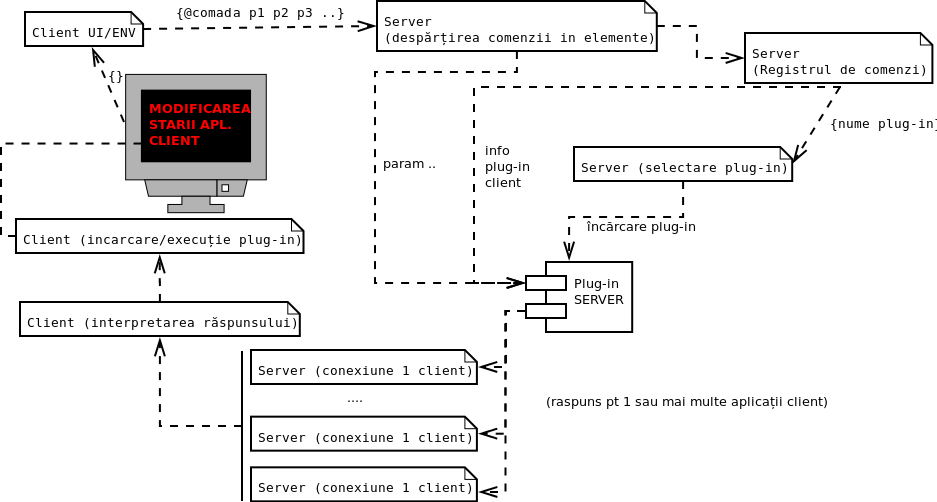
\includegraphics[scale=0.33]{loop}
    \caption{Bucla schimbului de informații între client și server}
    \label{fig:loop}
\end{figure}


\section{Diagrama claselor}
\begin{figure}[h]
    \centering
    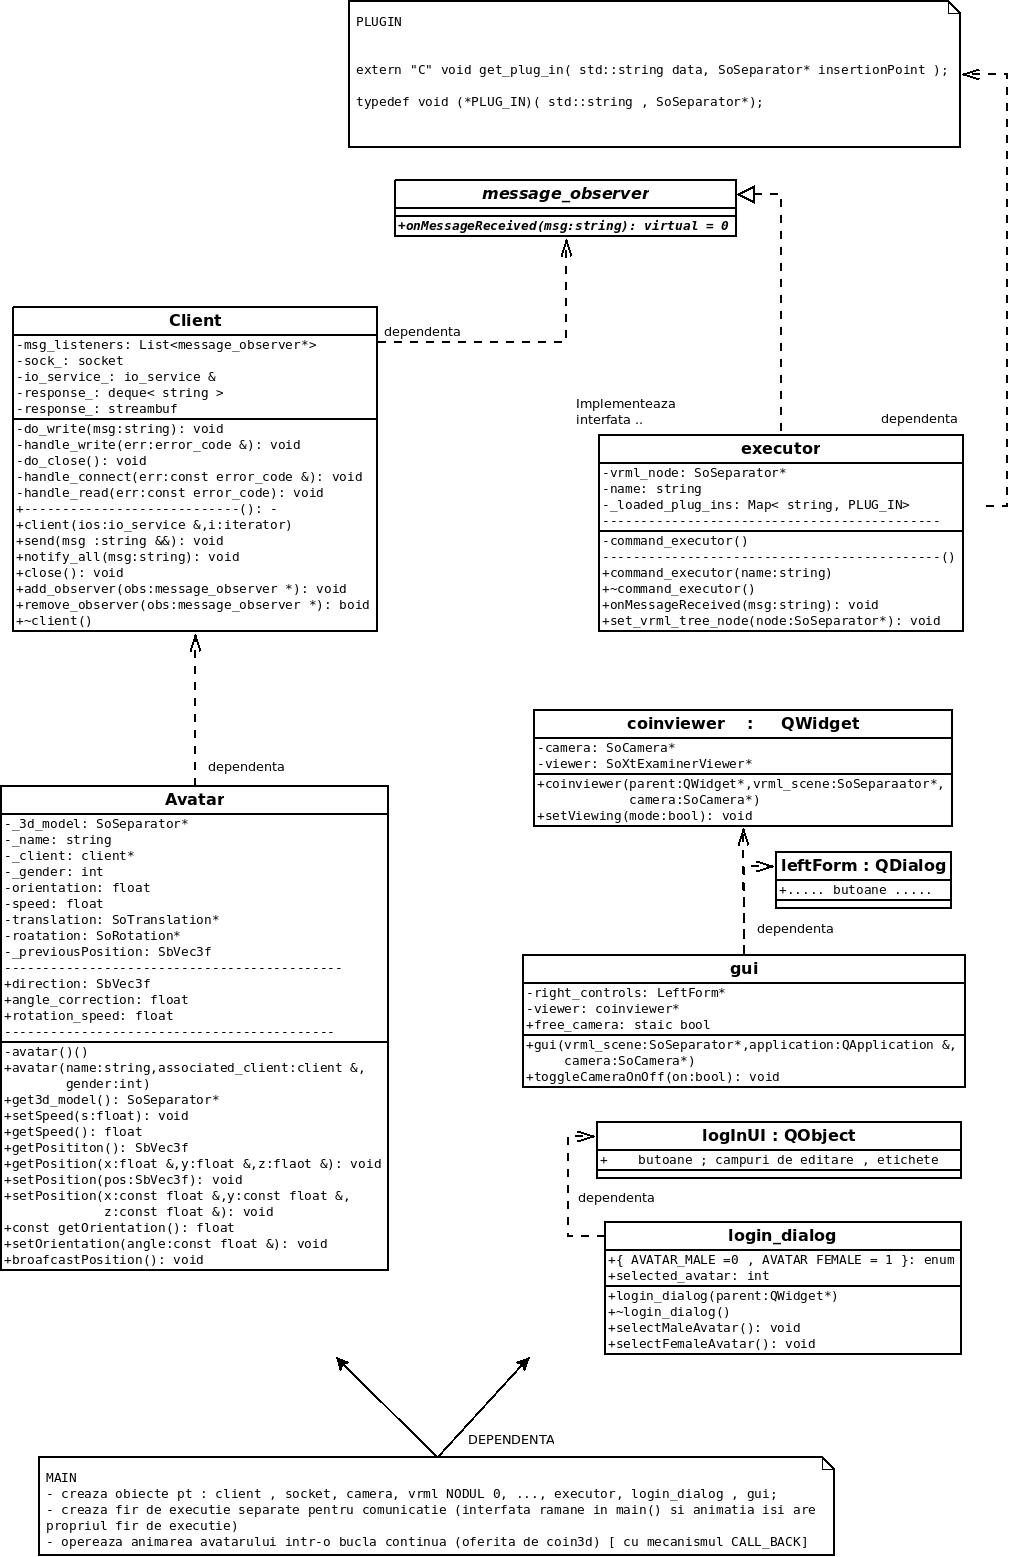
\includegraphics[scale=0.27]{UMLCL}
    \caption{Diagrama claselor aplicației client}
    \label{fig:loop}
\end{figure}

\section{Test}
\par Deoarece o metodă automată pentru testarea întregii aplicații este foarte complexă, se recurge la testarea vizuală, constând în verificarea modului în care perspectiva vizuală dintre două avatare este corectă, și în verificarea modului în care mediul virtual este redat din punct de vedere estetic.
\begin{figure}[ht]
    \centering
    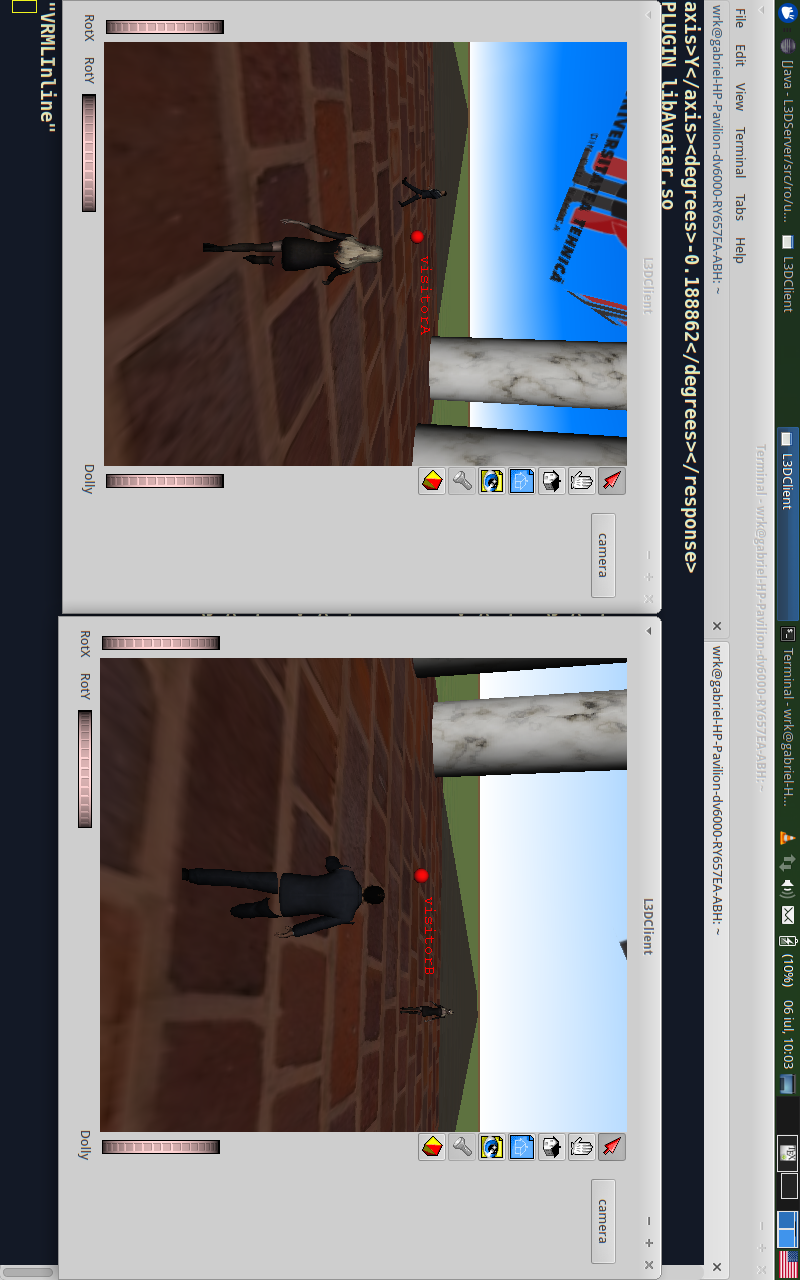
\includegraphics[scale=0.35]{CASTRUM0}
    \caption{Test - avatare - față în față }
    \label{fig:loop}
\end{figure}
\begin{figure}[ht]
    \centering
    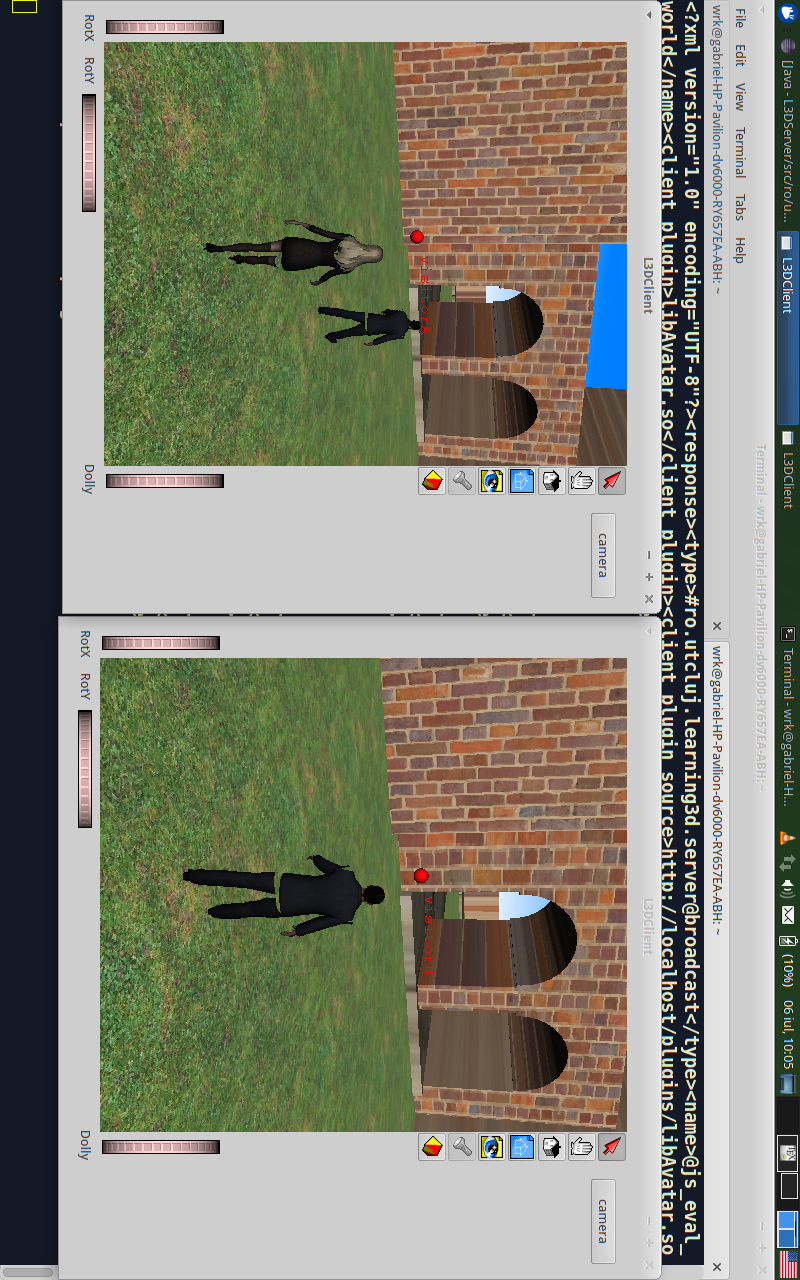
\includegraphics[scale=0.4]{P0}
    \caption{Test - avatare aliniate la intrarea într-o fortificație romană (3D)}
    \label{fig:loop}
\end{figure}
% \chapter{Conluzii}


\section{Conținut}

\begin{itemize}
 \item un rezumat al contribuțiilor aduse
 \item a analiză critică a rezultatelor obținute: avantaje, dezavantaje, limitări
 \item o descriere a posibilelor dezvoltări și îmbunătățiri ulterioare
\end{itemize}


\section{Detalii tehnice}

\subsection{Dimensiune}

Cca 3--5\% din total.





% \chapter{Concluzii}


\section{Instalarea bibliotecilor software}

\begin{itemize}
 \item un rezumat al contribuțiilor aduse
 \item a analiză critică a rezultatelor obținute: avantaje, dezavantaje, limitări
 \item o descriere a posibilelor dezvoltări și îmbunătățiri ulterioare
\end{itemize}


\section{Compilarea aplicației}

\subsection{Dimensiune}

Cca 3--5\% din total.






\appendix
\chapter{Testarea fiabilității modelului CLIENT-SERVER}
\section{Script}

\begin{verbatim}
#!/bin/bash

# seconds_EPOCH.sh

while read line

do
    echo $(date +%s) ":" $line;
done
\end{verbatim}
\par
\par ---------------------------------------------------------------------------------------
\par 
\begin{verbatim}
#!/bin/bash

# RUN_TESTS.sh

#!/bin/bash

telnetClients=10
rm ./*.out

echo "INCHIDEM SERVERUL ..."
kill -9 `pidof java` 
echo "START SERVER .... in 3 secunde "
java server &
sleep 3s
echo "OK" 

for ((1; i<=$telnetClients; ++i )) ; 
do
    fileName="./file_$i.out"
    telnet localhost 8080 | ./seconds_EPOCH.sh | tee -a $fileName &
done
\end{verbatim}

\section{Server de test}

\begin{lstlisting}
import java.net.ServerSocket;
import java.net.Socket;
import java.io.BufferedReader;
import java.io.IOException;
import java.io.InputStreamReader;
import java.io.PrintStream;
import java.util.ArrayList;

class SClient extends Thread {

    private Socket 		socket;
    private Integer 		serverId;
    private BufferedReader	istream;
    private PrintStream 	ostream;
    private boolean 		keepRunning;
    private static ArrayList<SClient> allServers = new ArrayList<SClient>();

    @SuppressWarnings("unused")
	private SClient() {
	// blocat
    }
	

    public SClient(Socket socket, Integer id) throws IOException {
		
	this.socket = socket;
	this.serverId = id;
	this.istream = new BufferedReader(new InputStreamReader(this.socket.getInputStream()));
	this.ostream = new PrintStream(socket.getOutputStream());
	this.keepRunning = true;
		
	allServers.add( this );
    }

    public void sendResponse(String response) {
	this.ostream.println(response);
    }
	
    private String getRequest() throws IOException {
	String line = "";

	try{
	    int c = 0;
	    while(((char)c)!='\n'){
		c= this.istream.read();
		line = line+(char)c;
		if(c==-1){
		    this.keepRunning = false;
		    break;
		}
	    }
	} catch (Exception e) {
	    e.printStackTrace();
	    this.keepRunning = false;
	}
		
	return line;
    }

    @Override
	public void run() {
	super.run();

	while(keepRunning) {
			
	    String text = "";
	    try {
		text = this.getRequest();
	    } catch (IOException e) {
		e.printStackTrace();
		text = "EROARE";
	    }
			
	    if ( text.contains("quit") || text.contains("exit") )
		{
		    System.exit(0);
		}

	    try{
			
		if ( allServers.size() >= 1 ) {
					
		    for(SClient user : allServers) {
			if(user!=null) {
			    user.sendResponse(text);
			}
		    }
		}
				
	    } catch (Exception e){
		e.printStackTrace();
		this.sendResponse("\nEROARE");
	    }
	}

	try {
	    this.socket.close();
	} catch (IOException e) {
	    e.printStackTrace();
	}
    }

}

/*

              serverul de test

*/

public class server {
	
    public static void main(String[] args){
		
	/*
	 *  in asteptarea clientilor
	 */
	int serverId=1;
	ServerSocket serverSocket;
	try {
	    serverSocket = new ServerSocket(8080);
	    for(;;){
		Socket s = serverSocket.accept();
		System.out.print("\nNew server [id="+serverId+"]");
		/*
		 *  client nou
		 */
		Thread t = new SClient(s, serverId);
		serverId++;
		t.start();
	    }
	} catch (IOException e) {
	    e.printStackTrace();
	}

    }
}

\end{lstlisting}


\subsection{Rezultate}
\par La verificarea diferențelor de timp la primirea datelor de către programele client cu comanda \textbf{ diff <fisier1> <fisier2> }. Testul este disponibil pentru verificare directorul ”Teste/ApendixA” în arhiva GIT a lucrării. Descărcarea se poate face cu comanda \textbf{git clone  https://github.com/gabrielchmod777/virtualWorldVRML-CLIENT.git}.

\par Testul este efectuat cu succes.





%\addcontentsline {toc}{chapter}{Bibliography}
\bibliographystyle{IEEEtran}
\bibliography{thesis}%same file name as for .bib

\end{document}
